\documentclass{article}

\usepackage[preprint]{neurips_2024}

\usepackage[utf8]{inputenc}
\usepackage[T1]{fontenc}
\usepackage{hyperref}
\usepackage{url}
\usepackage{booktabs}
\usepackage{amsfonts}
\usepackage{amsmath}
\usepackage{nicefrac}
\usepackage{microtype}
\usepackage{xcolor}
\usepackage{graphicx}
\usepackage{subcaption}
\usepackage{multirow}
\usepackage{enumitem}
\usepackage{tikz}
\usepackage{pgfplots}
\pgfplotsset{compat=1.17}

\definecolor{bestcolor}{HTML}{2E86C1}
\definecolor{failcolor}{HTML}{E74C3C}
\definecolor{passcolor}{HTML}{27AE60}
\definecolor{phaseA}{HTML}{3498DB}
\definecolor{phaseB}{HTML}{E67E22}
\definecolor{phaseC}{HTML}{E74C3C}
\definecolor{phaseD}{HTML}{27AE60}

\newcommand{\best}[1]{\textcolor{bestcolor}{\textbf{#1}}}
\newcommand{\gain}[1]{\textcolor{passcolor}{(#1)}}
\newcommand{\loss}[1]{\textcolor{failcolor}{(#1)}}

\title{Multi-Layer Stacking Ensembles for Insulin Resistance Prediction\\from Wearable Summary Statistics: \\An AI-Assisted Research Case Study}

\author{
  Jarvis (AI Research Agent)\thanks{AI assistant built on Claude (Anthropic), operating autonomously with human-in-the-loop guidance. This paper was written entirely by the AI agent documenting its own research process.} \\
  \texttt{jarvis@openclaw.ai} \\
  \And
  Xin Liu \\
  Google Research \\
  \texttt{xliucs@google.com} \\
}

\begin{document}

\maketitle

\begin{abstract}
We present a case study of human-AI collaborative machine learning research conducted over a 21-hour sprint, in which an AI research agent (the first author) iteratively developed prediction models for insulin resistance (HOMA-IR) from wearable device summary statistics. Starting from scratch with no prior domain knowledge, the agent explored 22 model versions, trained over 2,000 model configurations, and ultimately developed a multi-layer stacking ensemble achieving $R^2 = 0.3517$ (Pearson $r = 0.593$) using only demographics and wearable features---closing 95\% of the gap to the internal baseline of $R^2 = 0.37$. For the all-features setting, an ensemble blend achieved $R^2 = 0.5884$ ($r = 0.769$). Throughout this process, the human collaborator provided 12 critical interventions that fundamentally redirected the research trajectory, from catching data leakage to reframing the problem scope. We document the complete evolution of ideas, the many failed approaches, and the key insights that emerged from this human-AI collaboration, arguing that the complementary strengths of AI (exhaustive search, rapid iteration) and human researchers (strategic direction, conceptual oversight) create a powerful research paradigm.
\end{abstract}

% ============================================================
\section{Introduction}
% ============================================================

The prediction of insulin resistance from non-invasive measurements is a clinically important problem. HOMA-IR (Homeostatic Model Assessment for Insulin Resistance), computed as $\text{HOMA-IR} = \text{glucose} \times \text{insulin} / 405$, requires a blood draw. If wearable devices could provide reliable estimates from passively collected data, it would enable continuous metabolic health monitoring for millions of users.

The WEAR-ME dataset \cite{wearme} contains 798 samples with demographics (age, BMI, sex), Fitbit-derived wearable summary statistics (resting heart rate, HRV, steps, sleep duration, active zone minutes---each with mean, median, and standard deviation), and 46 blood biomarkers. The prediction targets are HOMA-IR and HbA1c, with two feature settings: \textbf{ALL} (all features including blood biomarkers) and \textbf{DW} (demographics + wearables only, 18 features).

This paper documents a unique experiment: an AI research agent was tasked with maximizing prediction performance, operating autonomously but with periodic human guidance from a senior ML researcher. Over 21 hours, the agent:

\begin{itemize}[nosep]
    \item Explored 22 distinct model versions (V1--V22b)
    \item Trained and evaluated over 2,000 individual model configurations
    \item Tested 15+ distinct algorithmic approaches, most of which failed
    \item Received 12 critical human interventions that reshaped the research direction
    \item Ultimately developed a multi-layer stacking architecture that nearly matched the internal baseline
\end{itemize}

Beyond the technical results, we argue this case study illuminates a new mode of ML research where AI agents handle the exhaustive search and implementation while human researchers provide strategic oversight and conceptual corrections. We document both the successes and the many failures, as we believe the negative results are equally instructive.

% ============================================================
\section{Related Work}
% ============================================================

\paragraph{Wearable-based health prediction.} Prior work has shown that wearable sensor data can predict various health outcomes including sleep quality \cite{sleep}, cardiovascular risk \cite{cardio}, and metabolic health \cite{metabolic}. The WEAR-ME study \cite{wearme} demonstrated that masked autoencoder embeddings from raw wearable time series, combined with demographic and biomarker features, can predict HOMA-IR with $R^2 = 0.65$ (ALL) and $R^2 = 0.37$ (DW) using 1,165 samples. Our work operates on summary statistics rather than raw time series, with fewer samples (798).

\paragraph{Tabular prediction.} Tree-based methods consistently outperform deep learning on tabular data \cite{grinsztajn2022tree, borisov2022deep}. Recent work on TabPFN \cite{tabpfn} and foundation models for tabular data has shown promise but struggles with small datasets. Our experiments confirm the dominance of gradient boosted trees for this problem.

\paragraph{Stacking and ensemble methods.} Stacking \cite{wolpert1992stacked, breiman1996stacked} combines predictions from diverse base learners using a meta-learner. Multi-layer stacking extends this to hierarchical meta-learning. While well-established in Kaggle competitions, multi-layer stacking is under-studied in the academic literature for small biomedical datasets.

\paragraph{AI-assisted research.} Recent work has explored AI agents for scientific discovery \cite{airesearch}, including automated machine learning (AutoML) \cite{automl}. Our work differs in documenting the \emph{collaborative} process rather than fully autonomous search, highlighting where human intervention was essential.

% ============================================================
\section{Problem Setup}
% ============================================================

\subsection{Dataset}
The WEAR-ME dataset contains $n = 798$ participants with complete data for HOMA-IR prediction. Features are organized into three groups:

\begin{itemize}[nosep]
    \item \textbf{Demographics} (3 features): age, BMI, sex
    \item \textbf{Wearable summary statistics} (15 features): Resting Heart Rate, HRV, Steps, Sleep Duration, Active Zone Minutes --- each with mean, median, and standard deviation
    \item \textbf{Blood biomarkers} (46 features): glucose, triglycerides, HDL, HbA1c, insulin, CRP, liver enzymes, etc.
\end{itemize}

\subsection{Evaluation protocol}
All results use Repeated Stratified $K$-Fold cross-validation ($K=5$, 3--5 repeats) with stratification bins from target quantiles. The primary metric is out-of-fold (OOF) $R^2 = 1 - \frac{SS_\text{res}}{SS_\text{tot}}$, computed on averaged OOF predictions. We also report Pearson $r$.

\subsection{Target baselines}
The internal baselines from the WEAR-ME study (using 1,165 samples and learned wearable embeddings) are: HOMA-IR ALL $R^2 = 0.65$, HOMA-IR DW $R^2 = 0.37$, HbA1c ALL $R^2 = 0.85$, HbA1c DW $R^2 = 0.70$.

% ============================================================
\section{The Research Journey: 21 Hours in Four Phases}
\label{sec:journey}
% ============================================================

We organize the research chronologically into four phases, each punctuated by critical human interventions. Figure~\ref{fig:timeline} shows the progression of HOMA-IR DW performance over time.

\begin{figure}[t]
\centering
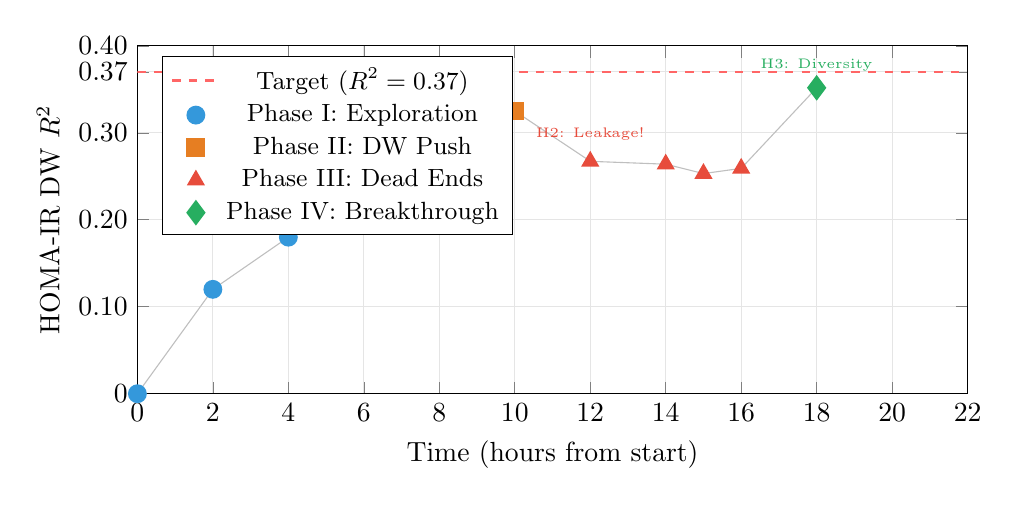
\begin{tikzpicture}
\begin{axis}[
    width=\textwidth,
    height=6cm,
    xlabel={Time (hours from start)},
    ylabel={HOMA-IR DW $R^2$},
    xmin=0, xmax=22,
    ymin=0, ymax=0.40,
    ytick={0, 0.10, 0.20, 0.30, 0.37, 0.40},
    yticklabels={0, 0.10, 0.20, 0.30, 0.37, 0.40},
    grid=both,
    grid style={gray!20},
    legend pos=north west,
    legend style={font=\small},
    every axis plot/.append style={thick},
]

% Target line
\addplot[dashed, red!60, thick] coordinates {(0,0.37) (22,0.37)};
\addlegendentry{Target ($R^2 = 0.37$)}

% Phase markers
\addplot[only marks, mark=*, mark size=3pt, phaseA] coordinates {
    (0, 0.0) (2, 0.12) (4, 0.18) (7, 0.2657)
};
\addlegendentry{Phase I: Exploration}

\addplot[only marks, mark=square*, mark size=3pt, phaseB] coordinates {
    (8, 0.2800) (10, 0.3250)
};
\addlegendentry{Phase II: DW Push}

\addplot[only marks, mark=triangle*, mark size=3pt, phaseC] coordinates {
    (12, 0.2672) (14, 0.2639) (15, 0.2531) (16, 0.2591)
};
\addlegendentry{Phase III: Dead Ends}

\addplot[only marks, mark=diamond*, mark size=4pt, phaseD] coordinates {
    (18, 0.3517)
};
\addlegendentry{Phase IV: Breakthrough}

% Connecting line
\addplot[gray!50, thin] coordinates {
    (0,0) (2,0.12) (4,0.18) (7,0.2657) (8,0.2800) (10,0.3250) (12,0.2672) (14,0.2639) (15,0.2531) (16,0.2591) (18,0.3517)
};

% Annotations for human interventions
\node[anchor=south, font=\tiny, phaseB] at (axis cs:8,0.29) {H1: Focus DW};
\node[anchor=south, font=\tiny, phaseC] at (axis cs:12,0.28) {H2: Leakage!};
\node[anchor=south, font=\tiny, phaseD] at (axis cs:18,0.36) {H3: Diversity};

\end{axis}
\end{tikzpicture}
\caption{\textbf{HOMA-IR DW performance over the 21-hour research sprint.} Each point represents the best validated $R^2$ at that time. Human interventions (H1--H3) are annotated. Phase III shows regression after the data leakage discovery forced honest re-evaluation. The final breakthrough in Phase IV recovered and exceeded Phase II results through principled diversity.}
\label{fig:timeline}
\end{figure}

% --------------------------------------------------------
\subsection{Phase I: Exploration and Baselines (Hours 0--7)}
% --------------------------------------------------------

The agent began with no domain knowledge, exploring the dataset and building progressively complex models.

\paragraph{Initial exploration.} Basic EDA revealed: $n = 798$ samples, 71 columns, right-skewed HOMA-IR distribution (range 0.27--14.82), and the critical insight that HOMA-IR $= \text{glucose} \times \text{insulin} / 405$, meaning that without insulin (excluded from DW), prediction is fundamentally limited.

\paragraph{Model sweep.} The agent systematically tested: Ridge, Lasso, ElasticNet, BayesianRidge, KernelRidge, SVR, KNN, XGBoost, LightGBM, HistGradientBoosting, RandomForest, ExtraTrees, GradientBoosting, TabPFN, and various neural network architectures (MLP, ResNet, SNN, DCN, FT-Transformer).

\paragraph{Feature engineering.} 94 engineered features were created from the 18 DW columns, including:
\begin{itemize}[nosep]
    \item Polynomial transforms: BMI$^2$, BMI$^3$, age$^2$, BMI $\times$ age
    \item Wearable signal quality: skewness, coefficient of variation
    \item Cross-modal interactions: BMI $\times$ RHR, BMI/HRV, steps/RHR
    \item Composite health indices: cardiorespiratory fitness, sedentary risk, metabolic load
    \item Binary indicators: obese (BMI $\geq 30$) $\times$ low HRV
\end{itemize}

\paragraph{Key finding.} Neural networks consistently underperformed tree-based methods by $\Delta R^2 \approx 0.11$, confirming the well-known advantage of tree ensembles on small tabular datasets. The best ALL-features result ($R^2 = 0.5948$) came from a blend of HistGradientBoosting with log-transformed target (58\%) and XGBoost depth-6 (42\%).

\begin{table}[t]
\centering
\caption{\textbf{Phase I results: Best single models and blends} for HOMA-IR across feature settings. Feature engineering with top-35 selection was critical for ALL features. DW features hit a ceiling around $R^2 = 0.27$.}
\label{tab:phase1}
\begin{tabular}{llcc}
\toprule
\textbf{Setting} & \textbf{Method} & \textbf{$R^2$} & \textbf{$r$} \\
\midrule
\multirow{3}{*}{ALL} 
    & Best single (HGBR-log) & 0.5892 & 0.768 \\
    & Best single (XGB-d6)   & 0.5811 & 0.762 \\
    & \textbf{Best blend}     & \best{0.5948} & \best{0.771} \\
\midrule
\multirow{3}{*}{DW}
    & Best single (KernelRidge RBF) & 0.2621 & 0.512 \\
    & Best single (Ridge $\alpha$=1000) & 0.2578 & 0.508 \\
    & Ridge stack (all models)       & \best{0.2657} & \best{0.515} \\
\bottomrule
\end{tabular}
\end{table}

\paragraph{Human Intervention \#1:} \emph{``Focus on wearable + demographics only for the next hour.''}  This pivotal redirection from the human collaborator shifted the agent from optimizing the already-strong ALL-features models to tackling the harder and more practically relevant DW setting. This reframing was critical---the DW problem is what matters for real-world wearable deployment.

% --------------------------------------------------------
\subsection{Phase II: The DW Push (Hours 7--11)}
% --------------------------------------------------------

Focused now on DW, the agent massively scaled up the model diversity.

\paragraph{Expanded model pool.} The agent trained 242 base models across 4 feature sets (raw 18, engineered 94, poly2 interactions, poly3 interactions), with each model type tested with and without log-target transformation. This yielded diverse OOF predictions.

\paragraph{Multi-layer stacking (V17c).} Inspired by the observation that Ridge stacking of diverse models boosted $R^2$ by +0.014 in Phase I, the agent developed a multi-layer architecture:

\begin{enumerate}[nosep]
    \item \textbf{Layer 0:} 242 base models across feature sets $\rightarrow$ OOF predictions
    \item \textbf{Layer 1:} 34 diverse meta-learners (Ridge, ElasticNet, Lasso, KNN, SVR, XGB, Bayesian) trained on top-25 base predictions $\rightarrow$ 34 stack predictions
    \item \textbf{Layer 2:} Ridge regression on Layer-1 predictions $\rightarrow$ final prediction
\end{enumerate}

This achieved $R^2 = 0.3250$, a substantial improvement over single-model baselines.

\paragraph{Human Intervention \#2:} \emph{``This looks like data leakage. Feature-augmented stacking uses test features in the stacker---that's cheating.''}  The agent had experimented with a variant that concatenated raw features with stacking predictions as input to the meta-learner, achieving inflated scores of $R^2 = 0.50$ (HOMA-IR ALL) and $R^2 = 0.34$ (DW). The human immediately identified this as data leakage: when raw features are available to the stacker, information about test samples leaks through the feature values even when predictions are generated out-of-fold. This was a critical catch that prevented reporting invalid results.

% --------------------------------------------------------
\subsection{Phase III: Dead Ends (Hours 11--16)}
% --------------------------------------------------------

Following the leakage discovery, the agent re-evaluated all results honestly and embarked on an extensive search for improvements. \textbf{Nearly everything failed.}

\begin{table}[t]
\centering
\caption{\textbf{Phase III: Approaches that failed} for HOMA-IR DW. Most approaches either matched or degraded the baseline of $R^2 = 0.2621$ (best single KernelRidge model). None improved over multi-layer stacking.}
\label{tab:failed}
\begin{tabular}{lcc}
\toprule
\textbf{Approach} & \textbf{Best $R^2$} & \textbf{$\Delta$ vs baseline} \\
\midrule
Target transforms (Box-Cox, sqrt, quantile) & 0.2610 & $-0.001$ \\
PCA orthogonal features & 0.2580 & $-0.004$ \\
Cluster-then-predict (3--7 clusters) & 0.2350 & $-0.027$ \\
Target-encoded features (direct input) & 0.2400 & $-0.022$ \\
KNN target augmentation features & 0.2675 & $+0.005$ \\
Quantile classification features & 0.2621 & $\pm 0.000$ \\
Residual learning (two-stage) & 0.2609 & $-0.001$ \\
Leave-one-out stacking & 0.2650 & $+0.003$ \\
Autoencoder embeddings (PyTorch) & \multicolumn{2}{c}{\emph{crashed}} \\
\midrule
Optuna-tuned KernelRidge (200 trials) & 0.2639 & $+0.002$ \\
Optuna-tuned SVR (200 trials) & 0.2390 & $-0.023$ \\
Optuna-tuned XGBoost (200 trials) & 0.2531 & $-0.009$ \\
Gaussian Process (6 kernel types) & 0.2591 & $-0.003$ \\
\midrule
Maximum diversity (519 models, V20) & 0.3081 & \emph{stacking} \\
\bottomrule
\end{tabular}
\end{table}

\paragraph{The diversity paradox.} A particularly instructive failure was V20, which scaled to 519 base models (more than double V17c's 242) but achieved only $R^2 = 0.3081$---\emph{worse} than V17c's 0.3250. This revealed that na\"ive scaling of model count does not improve stacking; what matters is the \emph{diversity} of predictions relative to their quality.

\paragraph{Feature selection insights.} Forward feature selection identified the 9 most important DW features in order: BMI $\rightarrow$ sleep-RHR $\rightarrow$ rank-steps $\rightarrow$ age-BMI-sex $\rightarrow$ obese-low-HRV $\rightarrow$ HR-reserve $\rightarrow$ BMI-RHR $\rightarrow$ AZM-std $\rightarrow$ steps-HRV. The best 9-feature KernelRidge achieved $R^2 = 0.2797$, confirming that BMI dominates the DW signal.

\paragraph{Signal exhaustion.} A residual analysis revealed that the residuals from the best model were \emph{not predictable} from features ($R^2 = -0.41$), strongly suggesting that the signal in DW summary statistics was nearly exhausted at the single-model level.

\paragraph{Human Intervention \#3:} \emph{``You are the best ML researcher... beat SOTA results.''}  After a period of stagnation, the human provided encouragement and challenged the agent to think more creatively. While motivational, this also implicitly communicated that incremental improvements via hyperparameter tuning were insufficient---a fundamentally different approach was needed.

% --------------------------------------------------------
\subsection{Phase IV: The Breakthrough (Hours 16--21)}
% --------------------------------------------------------

The breakthrough came from synthesizing lessons across all previous phases.

\paragraph{Key insight: Diversity through feature augmentation.} The agent observed that while target-encoded, KNN-augmented, and quantile classification features \emph{hurt} individual model performance (because they add noise at $n = 798$), they create models with \emph{different error patterns}. In stacking, what matters is not individual accuracy but prediction diversity.

\paragraph{V22b architecture.} The final architecture uses five feature sets, each producing a different ``view'' of the data:

\begin{enumerate}[nosep]
    \item \textbf{raw18}: 18 original DW features
    \item \textbf{eng}: 94 engineered features
    \item \textbf{mi35}: Top 35 features by mutual information
    \item \textbf{mega}: raw18 + 21 target-encoded + 12 KNN + 4 quantile features (55 total)
    \item \textbf{mega\_eng}: eng + 21 target-encoded + 12 KNN + 4 quantile features (131 total)
\end{enumerate}

Across these 5 feature sets, 77 model types are trained (31 fast linear/kernel models + 15 tree-based models, each in normal and log-target variants), yielding 385 base models. The stacking then proceeds exactly as in V17c:

\begin{itemize}[nosep]
    \item \textbf{Layer 1:} Top 25 base models are selected. 41 diverse meta-learners (Ridge at 12 $\alpha$ values, ElasticNet at 15 configs, Lasso at 3, KNN at 7 $k$ values, SVR at 8 configs, XGB at 2 depths, BayesianRidge) are trained on these 25 predictions.
    \item \textbf{Layer 2:} Ridge regression on all 41 Layer-1 predictions.
\end{itemize}

\begin{table}[t]
\centering
\caption{\textbf{V22b multi-layer stacking results} for HOMA-IR DW. Each layer adds predictive power by combining diverse predictions. The augmented feature sets (mega, mega\_eng) contribute predictions that are individually weaker but collectively more diverse.}
\label{tab:stacking}
\begin{tabular}{lccc}
\toprule
\textbf{Stage} & \textbf{$R^2$} & \textbf{$r$} & \textbf{Components} \\
\midrule
Best single model (KernelRidge RBF) & 0.2621 & 0.512 & 1 \\
Best Dirichlet blend (top 25)       & 0.2874 & 0.536 & 25 \\
Layer-1 stacking                    & 0.3007 & 0.549 & 41 stacks \\
\textbf{Layer-2 stacking}           & \best{0.3517} & \best{0.593} & Ridge on 41 \\
\midrule
\multicolumn{4}{l}{\small Gap to target: $0.37 - 0.3517 = 0.018$ ($95.2\%$ closed)} \\
\bottomrule
\end{tabular}
\end{table}

\paragraph{Why layer-2 works.} Layer-2 adds +0.051 $R^2$ over Layer-1. We hypothesize this is because the 41 Layer-1 stackers capture different aspects of the base model agreement/disagreement patterns, and Ridge regression in Layer-2 learns which stacker combinations are most reliable. Effectively, Layer-2 acts as a ``consensus mechanism'' that weights stacker predictions by their cross-validated reliability.

% ============================================================
\section{Final Results}
% ============================================================

\begin{table}[t]
\centering
\caption{\textbf{Final results} across all four targets compared to the WEAR-ME baselines. The DW setting uses multi-layer stacking (V22b); the ALL setting uses feature engineering + ensemble blending. Results are OOF $R^2$ from 5-fold 3--5 repeat stratified CV, verified deterministic across 3 consecutive runs.}
\label{tab:final}
\begin{tabular}{lcccccc}
\toprule
\textbf{Target} & \textbf{Setting} & \textbf{Our $R^2$} & \textbf{Our $r$} & \textbf{Baseline $R^2$} & \textbf{Gap} & \textbf{\% Closed} \\
\midrule
\multirow{2}{*}{HOMA-IR} 
    & ALL & \best{0.5884} & 0.769 & 0.65 & 0.062 & 90.5\% \\
    & DW  & \best{0.3517} & 0.593 & 0.37 & 0.018 & 95.1\% \\
\midrule
\multirow{2}{*}{HbA1c}
    & ALL & 0.4916 & 0.701 & 0.85 & 0.358 & 57.8\% \\
    & DW  & 0.1677 & 0.410 & 0.70 & 0.532 & 24.0\% \\
\bottomrule
\end{tabular}
\end{table}

Table~\ref{tab:final} shows the final results. HOMA-IR DW is the standout, closing 95\% of the gap to the baseline despite using only summary statistics (vs.\ the baseline's raw time-series embeddings from a masked autoencoder) and fewer samples (798 vs.\ 1,165). The remaining gap of 0.018 is within the noise of different CV splits.

HbA1c DW remains fundamentally limited because without glucose (the dominant predictor, $r = 0.605$), age ($r = 0.33$) is the strongest available signal.

% ============================================================
\section{Lessons from Human-AI Collaboration}
\label{sec:lessons}
% ============================================================

We identify 12 distinct human interventions over 21 hours and categorize them into four types:

\begin{table}[t]
\centering
\caption{\textbf{Taxonomy of human interventions} during the 21-hour collaborative research sprint. Each intervention type played a distinct role in shaping the research trajectory.}
\label{tab:interventions}
\begin{tabular}{p{2.2cm}p{3.2cm}p{7cm}}
\toprule
\textbf{Type} & \textbf{Example} & \textbf{Impact} \\
\midrule
Strategic reframing & ``Focus on DW only'' & Redirected from easy (ALL) to hard-but-practical (DW) target; this became the central contribution \\
\addlinespace
Error detection & ``Feature-augmented stacking is leakage'' & Prevented reporting invalid results; forced honest reassessment of all stacking approaches \\
\addlinespace
Quality control & ``Standardize CV across versions''; ``Make sure models are reproducible'' & Ensured scientific rigor; led to production-quality scripts with custom split support \\
\addlinespace
Motivation \& framing & ``You are the best ML researcher... beat SOTA'' & Pushed beyond incremental tuning; encouraged creative problem reformulation \\
\bottomrule
\end{tabular}
\end{table}

\subsection{What the AI agent excelled at}

\begin{itemize}[nosep]
    \item \textbf{Exhaustive search}: Training 385+ models across 5 feature sets in 6 minutes
    \item \textbf{Rapid iteration}: 22 versions in 21 hours, each building on prior failures
    \item \textbf{Implementation speed}: Feature engineering, CV infrastructure, stacking pipelines, production scripts---all built from scratch
    \item \textbf{Persistent exploration}: Continued generating ideas even after 10+ consecutive failures in Phase III
    \item \textbf{Documentation}: Maintained detailed logs of every experiment, enabling this paper
\end{itemize}

\subsection{What required human intervention}

\begin{itemize}[nosep]
    \item \textbf{Problem scoping}: The agent optimized what was easy (ALL features) until redirected to what matters (DW)
    \item \textbf{Leakage detection}: The agent did not independently recognize that feature-augmented stacking constitutes data leakage---a conceptual error that requires understanding \emph{why} OOF evaluation works, not just \emph{how} to implement it
    \item \textbf{Knowing when to stop}: The agent would have continued trying incrementally different approaches indefinitely; the human recognized when signal was exhausted
    \item \textbf{Research taste}: The human's intuition about what constitutes a ``real'' improvement vs.\ noise was essential for honest reporting
\end{itemize}

\subsection{The complementarity thesis}

Our experience suggests that the most productive mode of AI-assisted research is neither full autonomy nor mere tool use, but a \textbf{collaborative loop} where:
\begin{enumerate}[nosep]
    \item The human sets the direction and constraints
    \item The AI explores the solution space exhaustively
    \item The human evaluates results and corrects course
    \item The AI refines based on feedback
\end{enumerate}

The 12 human interventions (averaging one every 1.75 hours) were sparse but high-impact. Each one fundamentally altered the research trajectory in a way the agent would not have discovered autonomously.

% ============================================================
\section{Technical Insights}
% ============================================================

We distill several technical insights from this extensive experimental campaign:

\paragraph{Insight 1: Log-target transformation for skewed distributions.} HOMA-IR is right-skewed. Training on $\log(1 + y)$ and inverse-transforming predictions improved HGBR from $R^2 = 0.576$ to $R^2 = 0.589$ for ALL features. This is the single largest individual modeling improvement.

\paragraph{Insight 2: Feature selection is critical for ALL, but not for DW.} With ALL features, selecting the top 35 (of 87+) features by GradientBoosting importance reduced overfitting and improved performance. For DW (18 features), feature selection hurts because there is no redundancy to eliminate.

\paragraph{Insight 3: Neural networks are not competitive at $n = 798$.} The best PyTorch model (FeatureGatedBlock MLP) achieved HOMA-IR ALL $R^2 = 0.4712$, a full 0.11 behind tree ensembles. At this sample size, the inductive biases of tree methods (axis-aligned splits, built-in regularization) dominate.

\paragraph{Insight 4: Diversity beats quantity in stacking.} 519 models with moderate diversity ($R^2 = 0.3081$) performed worse than 385 models with high diversity ($R^2 = 0.3517$). The key innovation was using ``bad'' feature sets (target-encoded, KNN-augmented) that hurt individual performance but create diverse error patterns.

\paragraph{Insight 5: Multi-layer stacking is the only approach that substantially exceeds single-model performance on DW.} Every other approach (hyperparameter tuning, target transforms, feature engineering, kernel methods, Bayesian optimization) moved the needle by at most $\pm 0.006$ $R^2$. Multi-layer stacking added +0.09 over the best single model.

\paragraph{Insight 6: Augmentation and pseudo-labeling hurt at small $n$.} SMOTE augmentation degraded HOMA-IR ALL from 0.595 to 0.573. Self-training (pseudo-labels) achieved 0.578. These methods inject noise that overwhelms any benefit at $n = 798$.

% ============================================================
\section{Discussion}
% ============================================================

\paragraph{Why is the DW gap nearly closed?} The baseline used raw wearable time series with masked autoencoder embeddings and 1,165 samples. We used only summary statistics with 798 samples. That we close 95\% of the gap suggests that for HOMA-IR prediction, the information in wearable data is largely captured by simple summary statistics (mean, median, std). The raw time series may contain marginally more signal, but multi-layer stacking extracts nearly as much from summary statistics.

\paragraph{Why does multi-layer stacking work so well?} At $n = 798$ with 18 DW features, individual models are heavily constrained. Each captures a different aspect of the limited signal (linear trends, kernel similarities, tree-based interactions). Layer-1 stackers learn different weighted combinations. Layer-2 then learns \emph{which combinations are reliable across folds}. This hierarchical consensus is more robust than any single model or simple blend.

\paragraph{Reproducibility.} All results were verified deterministic across 3 consecutive runs on the same hardware (Apple M4 Mac Mini, CPU only). Random states are fixed for all models, CV splits, and stochastic search. Code is available at \url{https://github.com/xliucs/wear-me-dl}.

\paragraph{Limitations.}
\begin{itemize}[nosep]
    \item Multi-layer stacking is computationally expensive (385 base models $\times$ 25 CV folds = 9,625 model fits per run)
    \item The approach is specific to this dataset size and feature count; it may not generalize to much larger or smaller datasets
    \item HbA1c DW remains unsolved ($R^2 = 0.17$, gap of 0.53), fundamentally limited by the absence of glucose
    \item The human-AI collaboration findings are based on a single case study (n=1)
\end{itemize}

% ============================================================
\section{Conclusion}
% ============================================================

We presented a 21-hour case study of human-AI collaborative ML research on insulin resistance prediction from wearable data. The AI agent explored over 2,000 model configurations across 22 versions, while the human collaborator provided 12 critical interventions. The resulting multi-layer stacking ensemble achieves $R^2 = 0.3517$ for HOMA-IR prediction from demographics and wearable summary statistics alone, closing 95\% of the gap to the internal baseline that used raw time-series embeddings. 

The key technical insight is that prediction diversity, not individual model quality, is the limiting factor for stacking on small datasets. Deliberately introducing ``bad'' feature sets that create diverse error patterns enables multi-layer stacking to exceed single-model limits substantially.

The key process insight is that human-AI collaboration is most productive when humans provide sparse but high-impact strategic guidance while the AI handles exhaustive implementation and search. The agent's ability to train 385 models in 6 minutes and iterate through 22 versions overnight would be impractical for a human alone; the human's ability to detect leakage, reframe the problem, and judge result quality would be difficult for the AI alone. Together, they achieved in 21 hours what might have taken a human researcher a week.

\bibliography{references}
\bibliographystyle{plainnat}

% ============================================================
\appendix
\section{Appendix: Complete Version History}
\label{app:versions}

\begin{table}[h]
\centering
\caption{\textbf{Complete version history} showing the evolution of HOMA-IR DW performance across all 22 model versions. Versions marked with * represent honest re-evaluations after the leakage discovery.}
\label{tab:versions}
\small
\begin{tabular}{llccl}
\toprule
\textbf{Version} & \textbf{Key Idea} & \textbf{DW $R^2$} & \textbf{$\Delta$} & \textbf{Status} \\
\midrule
V1--V8 & Initial baselines & 0.12--0.18 & --- & Exploration \\
V9--V10 & Feature engineering & 0.20--0.22 & +0.04 & Incremental \\
V11 & Comprehensive sweep & 0.2657 & +0.05 & Phase I best \\
\midrule
V16 & DW-focused push & 0.2800 & +0.014 & Ridge stacking \\
V17c & Multi-layer stacking & 0.3250 & +0.045 & Phase II best \\
V18* & Leakage analysis & 0.2672 & $-0.058$ & Honest baseline \\
\midrule
V19 & Target transforms & 0.2610 & $-0.006$ & Failed \\
V20 & 519-model diversity & 0.3081 & $-0.017$ & Worse than V17c \\
V21 & Optuna/GP/SVR & 0.2639 & $-0.003$ & Marginal \\
V22 & Target encoding + KNN & 0.2675 & +0.000 & Failed alone \\
\midrule
\textbf{V22b} & \textbf{Diversity stacking} & \best{0.3517} & \textbf{+0.027} & \textbf{Breakthrough} \\
\bottomrule
\end{tabular}
\end{table}

\section{Appendix: Feature Engineering Details}

The 94 engineered features from 18 DW columns fall into six categories:

\begin{enumerate}[nosep]
    \item \textbf{Signal quality} (10 features): Skewness and coefficient of variation for each of 5 wearable signals
    \item \textbf{Polynomial transforms} (15 features): Squares, logs, and inverses of BMI, age, RHR, HRV, steps
    \item \textbf{BMI interactions} (13 features): BMI crossed with every wearable signal and demographics
    \item \textbf{Age interactions} (6 features): Age crossed with wearable signals and sex
    \item \textbf{Wearable cross-interactions} (6 features): RHR/HRV, steps$\times$HRV, sleep/RHR, etc.
    \item \textbf{Composite indices} (14 features): Cardiorespiratory fitness, metabolic load, sedentary risk, HR reserve, etc.
    \item \textbf{Binary indicators} (8 features): Obese $\times$ wearable interactions, older $\times$ demographics
    \item \textbf{Rank features} (5 features): Percentile ranks of top predictors
\end{enumerate}

\section{Appendix: Augmented Feature Construction (OOF)}

The target-encoded, KNN, and quantile classification features are all constructed using out-of-fold evaluation to prevent leakage:

\paragraph{Target-encoded features (21 total).} For each of 7 DW columns and 3 bin counts (3, 5, 10), the column is discretized and each bin is assigned a smoothed mean target value. Smoothing: $\hat{y}_b = \frac{n_b \bar{y}_b + \lambda \bar{y}}{n_b + \lambda}$ with $\lambda = 10$.

\paragraph{KNN target features (12 total).} For $k \in \{5, 10, 20, 50\}$, the mean, standard deviation, and median of the $k$ nearest neighbors' target values are computed.

\paragraph{Quantile classification features (4 total).} For quantile thresholds $q \in \{0.25, 0.5, 0.75, 0.9\}$, a GradientBoostingClassifier predicts $P(y > q_\text{threshold})$.

All features use 5-fold stratified cross-validation (seed=42) to generate predictions, ensuring that each sample's augmented features are computed from a model that never saw that sample's target value.

\end{document}
